The flavor rescaling corrects the under-estimation of the $\ttbar+HF$ production rate in the MC prediction. This is performed by rescaling the normalization of $\ttbar+light$ (TTL), $\ttbar+\ge 1c$ (TTC) and $\ttbar+\ge 1b$ (TTB). The scale factors are derived by performing a likelihood fit on the sum of the pseudo continuous b-tagged score (pcb) of the third and forth jets ranked in DL1r score, as this variable is highly sensitive to the $\ttbar+HF$ samples. A combined fit is performed in 7j region from the 1L channel and 5j region from the OS channel with $=2b$, $=3b$ and $\geq 4b$ requirements, where the signal contamination of all the signal mass points is around or smaller than $0.1\%$. The normalisation of TTL, TTC and TTB are free floating in this fit, and that TTL normalisation for 1L and 2LOS are treated as two independent normalisaiton factors. The nominal \ttbar sample is used for this fit. The nuisance parameters associated to the systematic uncertainties on the b-tagging efficiency (as described in Section~\ref{b-tagging_uncertianties}) and the cross-section uncertainties of other backgrounds, which cannot be neglected in the fitting regions, are fitted together with the correction factors of TTL, TTC and TTB because these uncertainties highly affect the yields of $\ttbar+HF$ and other backgrounds.

% as given in the Table~\ref{tab:HF_postFit_nominal}

\begin{table}[th!]
    \centering
    \def\arraystretch{1.2}
    \resizebox*{0.3\textwidth}{!}{
    \begin{tabular}{c|cc}
        \toprule
          & 1L & OS \\
          & $=7j$ & $=5j$ \\
        \hline
         2b & $<0.1\%$ & $<0.1\%$ \\
         3b & $<0.1\%$ & $<0.1\%$ \\
         $\geq4b$ & $0.2\%$ & $0.1\%$ \\
        \bottomrule
    \end{tabular}
    }
    \caption{\label{tab:sigContam_HFCorrRegion}The signal (BSMtttt M700) over background ratio in each of the regions used to derive the HF rescaling factors before any scaling applied.}
\end{table}

The pre-fit and post-fit distributions of the third and the forth jets pcb sum in 1L and OS channels can be found in figure~\ref{fig:1L_pcb34_PrePost} and~\ref{fig:2LOS_pcb34_PrePost} respectively. The pre-fit and post-fit summary plots, which show the yields in each region, in both channel can be found in figure~\ref{fig:HF_summaryPlot} while the fitted normalization factors and nuisance parameters can be found in figure~\ref{fig:HF_scale_fit}. The obtained normalization factors are consistent with other ATLAS analyses targeting similar phase space. For example, the ttH(bb) measurement \cite{HIGG-2017-03} found tt+b and tt+c normalization factors of 1.24 and 1.63, respectively. Most of the nuisance parametrs are neither pulled nor constrained. However, when the fits are done separately on two channels, it is observed that both nuisance parameters of c-tagging EV0 and light-tagging EV0 are pulled in oposite direction between two channels. Therefore these two nuisance parameters are decorrelated from the two channels in the combined fit.
It is also found that having the combined fit in TTL scale factor causes the inconsistent results with the 1L and OS channel separated fit, because the acceptance of the TTL events between these two channel are different. To keep a stable fit results, the TTL correction factors are derived on separate channels during the combined fit.



\begin{figure}[!htb]
    \centering
    \subfloat[1L$(=7j,=2b)$ Pre-fit]{
        
\includegraphics[height=0.3\textheight]{plots/bkg_modelling/HF_scaling/pcbSum34_ljets_7j2b_preFit.pdf}
    }
    \subfloat[1L$(=7j,=2b)$ Post-Fit]{
        
\includegraphics[height=0.3\textheight]{plots/bkg_modelling/HF_scaling/pcbSum34_ljets_7j2b_postFit.pdf}
    }

    \subfloat[1L$(=7j,=3b)$ Pre-fit]{
        
\includegraphics[height=0.3\textheight]{plots/bkg_modelling/HF_scaling/pcbSum34_ljets_7j3b_preFit.pdf}
    }
    \subfloat[1L$(=7j,=3b)$ Post-Fit]{
        
\includegraphics[height=0.3\textheight]{plots/bkg_modelling/HF_scaling/pcbSum34_ljets_7j3b_postFit.pdf}
    }
    
    \subfloat[1L$(=7j,\geq 4b)$ Pre-fit]{
        
\includegraphics[height=0.3\textheight]{plots/bkg_modelling/HF_scaling/pcbSum34_ljets_7jge4b_preFit.pdf}
    }
    \subfloat[1L$(=7j,\geq 4b)$ Post-Fit]{
        
\includegraphics[height=0.3\textheight]{plots/bkg_modelling/HF_scaling/pcbSum34_ljets_7jge4b_postFit.pdf}
    }
    \caption{\label{fig:1L_pcb34_PrePost}The pre-fit (left) and post-fit (right) distributions of pcb sum of the third and the forth jets at 7j region with $=2b$, $=3b$ and $\geq 4b$ in 1L channel to derive the HF scale factor.}
\end{figure}


\begin{figure}[!htb]
    \centering
    \subfloat[1L$(=5j,=2b)$ Pre-fit]{
        
\includegraphics[height=0.3\textheight]{plots/bkg_modelling/HF_scaling/pcbSum34_os2l_5j2b_preFit.pdf}
    }
    \subfloat[1L$(=5j,=2b)$ Post-Fit]{
        
\includegraphics[height=0.3\textheight]{plots/bkg_modelling/HF_scaling/pcbSum34_os2l_5j2b_postFit.pdf}
    }

    \subfloat[1L$(=5j,=3b)$ Pre-fit]{
        
\includegraphics[height=0.3\textheight]{plots/bkg_modelling/HF_scaling/pcbSum34_os2l_5j3b_preFit.pdf}
    }
    \subfloat[1L$(=5j,=3b)$ Post-Fit]{
        
\includegraphics[height=0.3\textheight]{plots/bkg_modelling/HF_scaling/pcbSum34_os2l_5j3b_postFit.pdf}
    }

    \subfloat[1L$(=5j,\geq 4b)$ Pre-fit]{
        
\includegraphics[height=0.3\textheight]{plots/bkg_modelling/HF_scaling/pcbSum34_os2l_5jge4b_preFit.pdf}
    }
    \subfloat[1L$(=5j,\geq 4b)$ Post-Fit]{
        
\includegraphics[height=0.3\textheight]{plots/bkg_modelling/HF_scaling/pcbSum34_os2l_5jge4b_postFit.pdf}
    }
    \caption{\label{fig:2LOS_pcb34_PrePost}The pre-fit (left) and post-fit (right) distributions of pcb sum of the third and the forth jets at 5j region with $=2b$, $=3b$ and $\geq 4b$ in OS channel to derive the HF scale factor.}
\end{figure}

\begin{figure}[ht!]
  \centering
    \begin{subfigure}[t]{\textwidth}
        \centering
        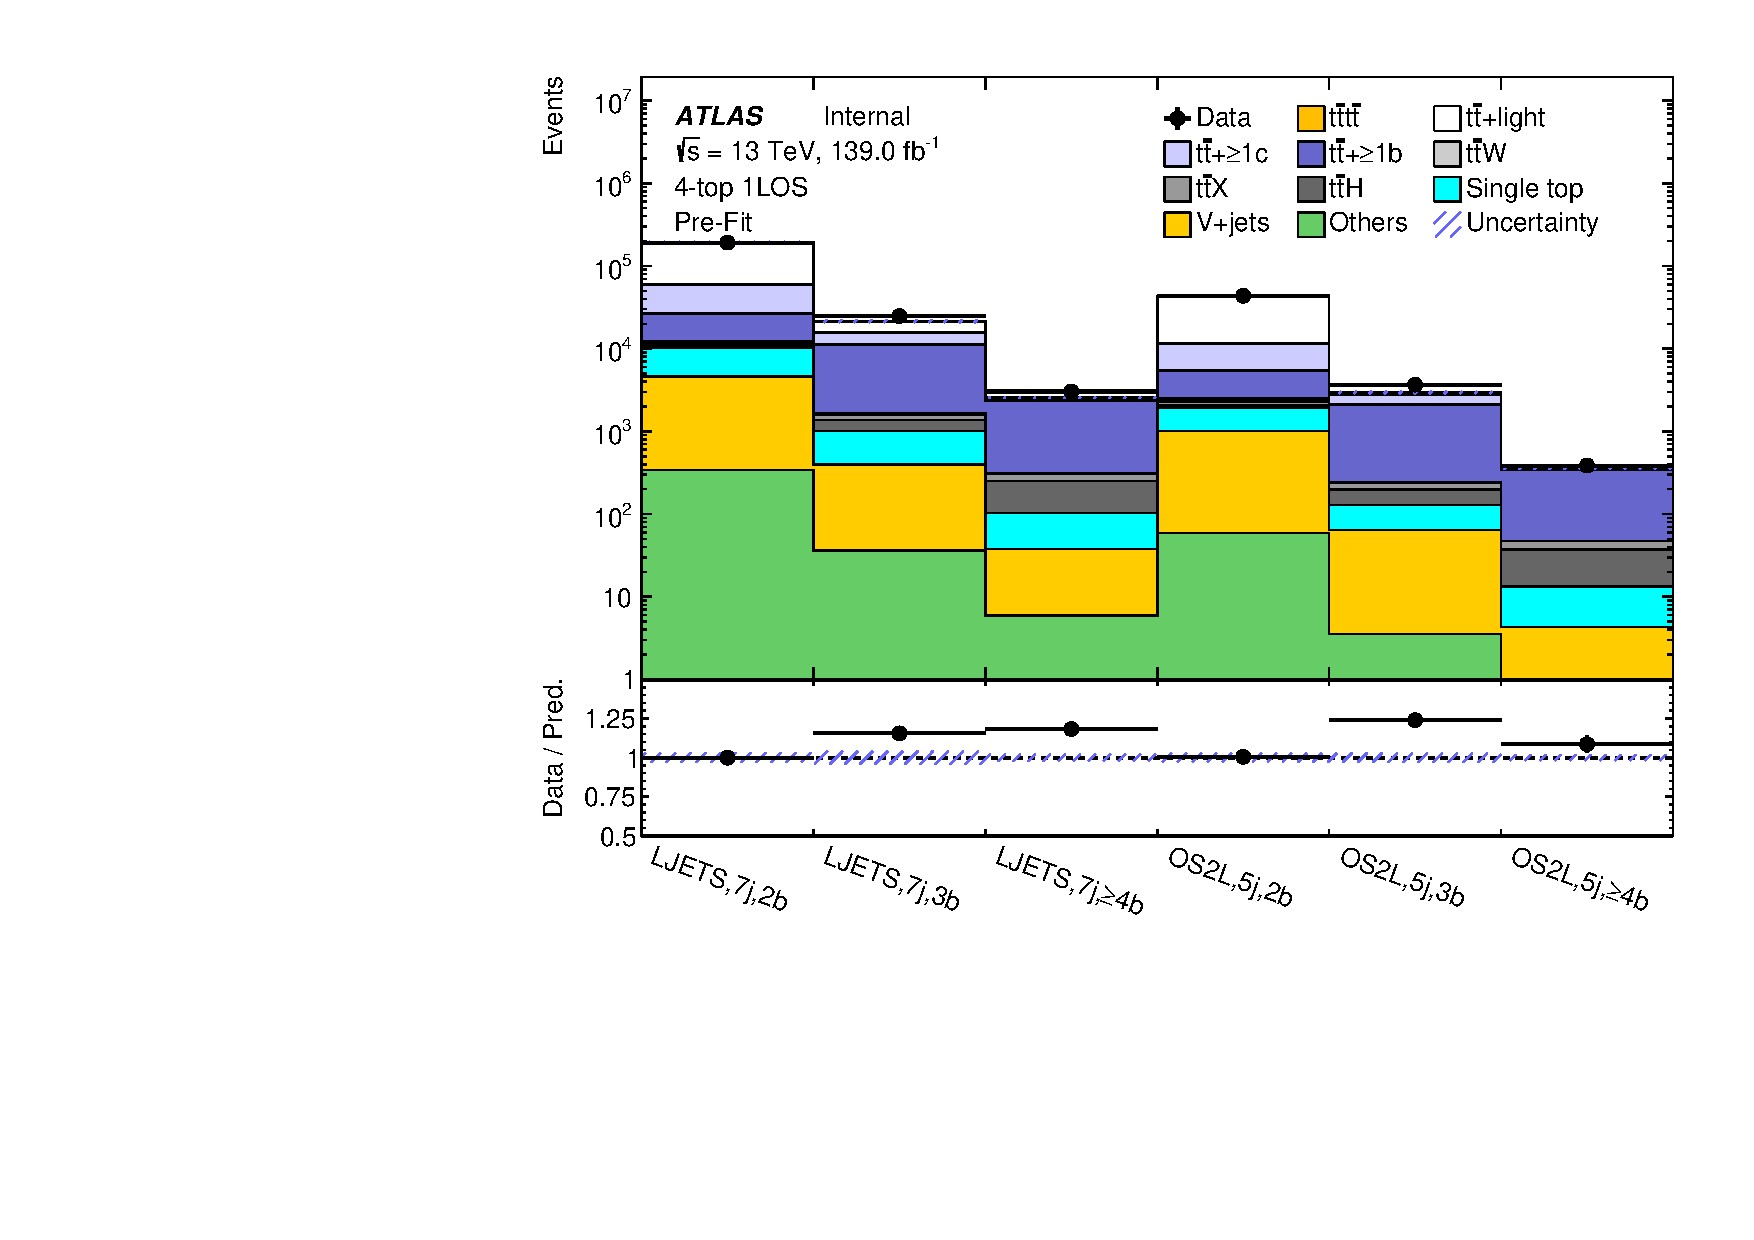
\includegraphics[width=0.48\textwidth]{plots/bkg_modelling/HF_scaling/Summary_preFit.pdf}
        
\includegraphics[width=0.48\textwidth]{plots/bkg_modelling/HF_scaling/Summary_postFit.pdf}
    \end{subfigure}
    \caption{Pre-fit (left) and post-fit (right) distributions of the yields in the regions included in the fit to determine HF scale factors.}
    \label{fig:HF_summaryPlot}
\end{figure}

\begin{figure}[ht!]
  \centering
    \begin{subfigure}[t]{\textwidth}
        \centering
        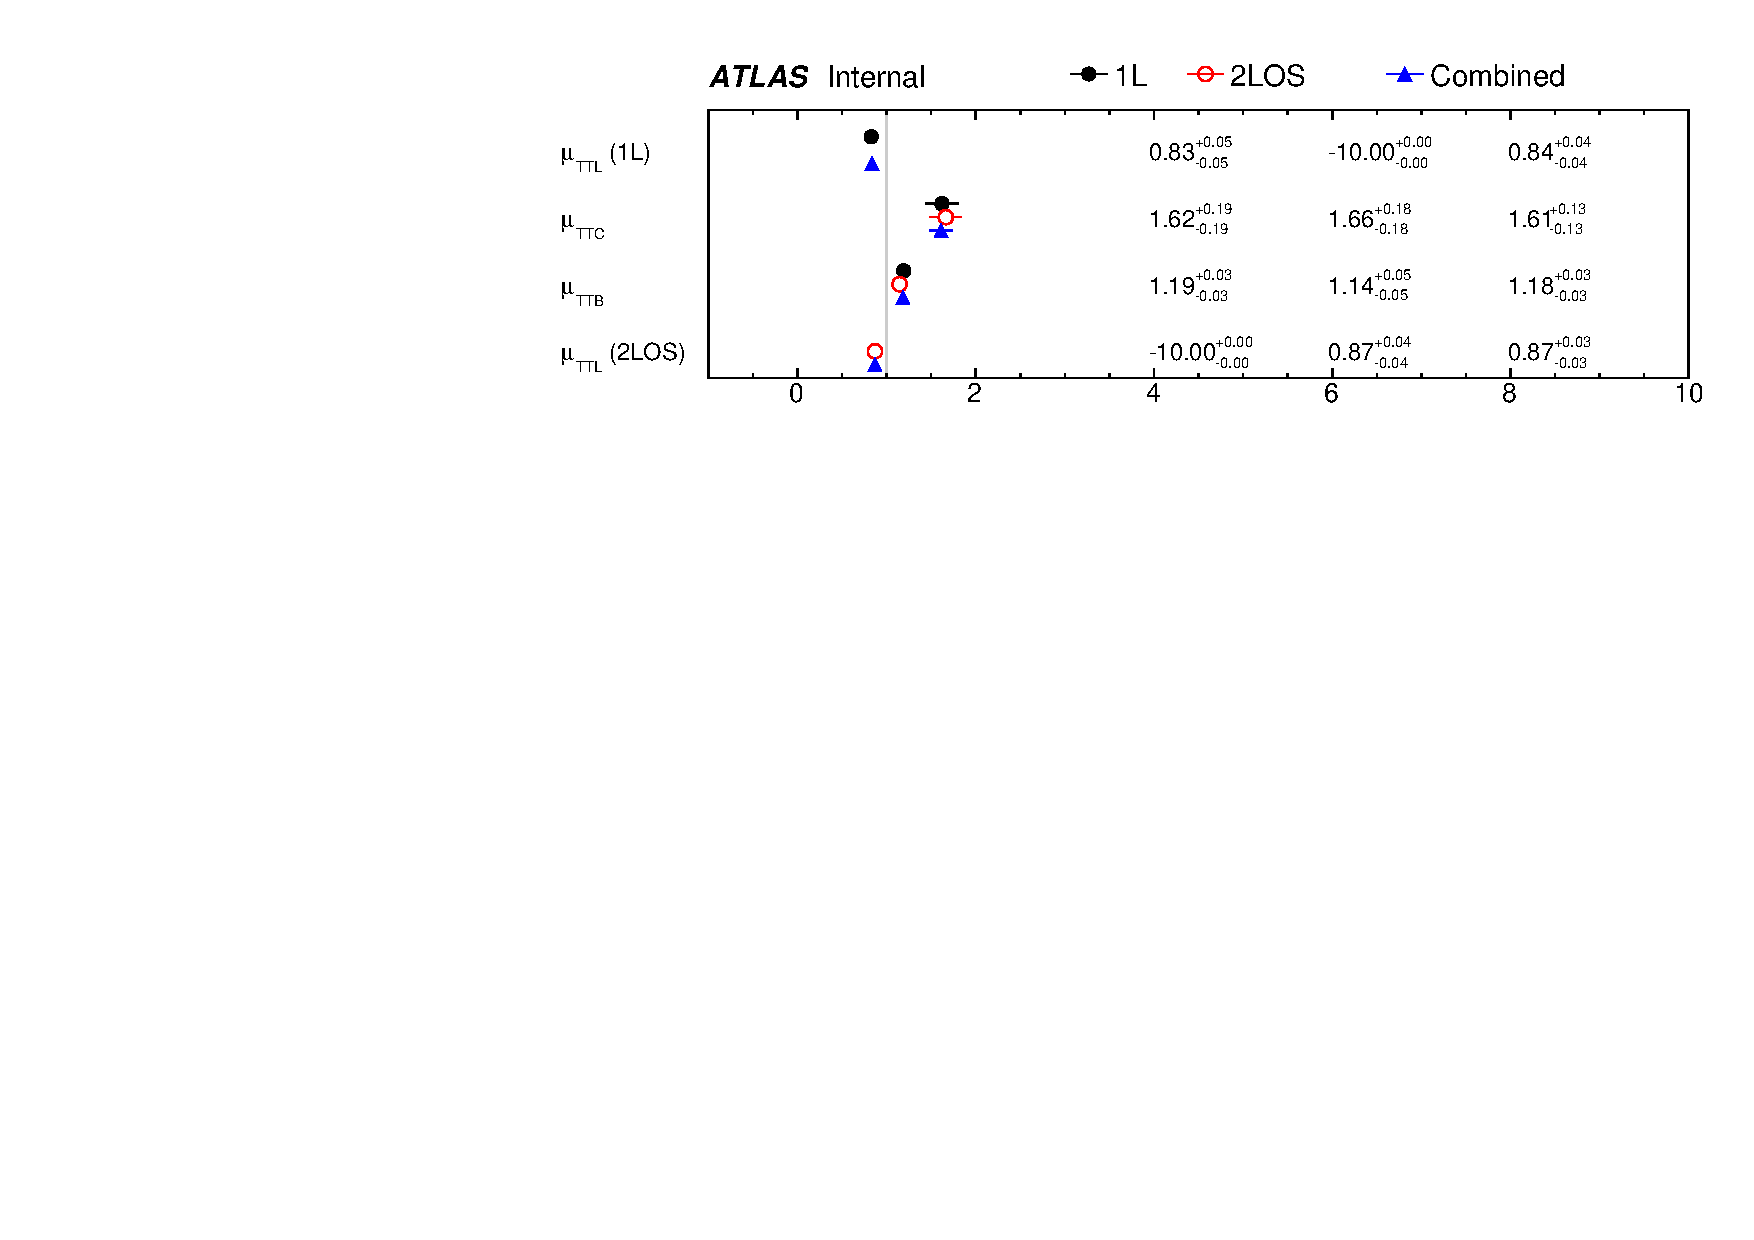
\includegraphics[width=0.78\textwidth]{plots/bkg_modelling/HF_scaling/NormFactors_multiFit.pdf}
    \end{subfigure}
    \bigskip
    \centering
    \begin{subfigure}[t]{\textwidth}
        \centering
        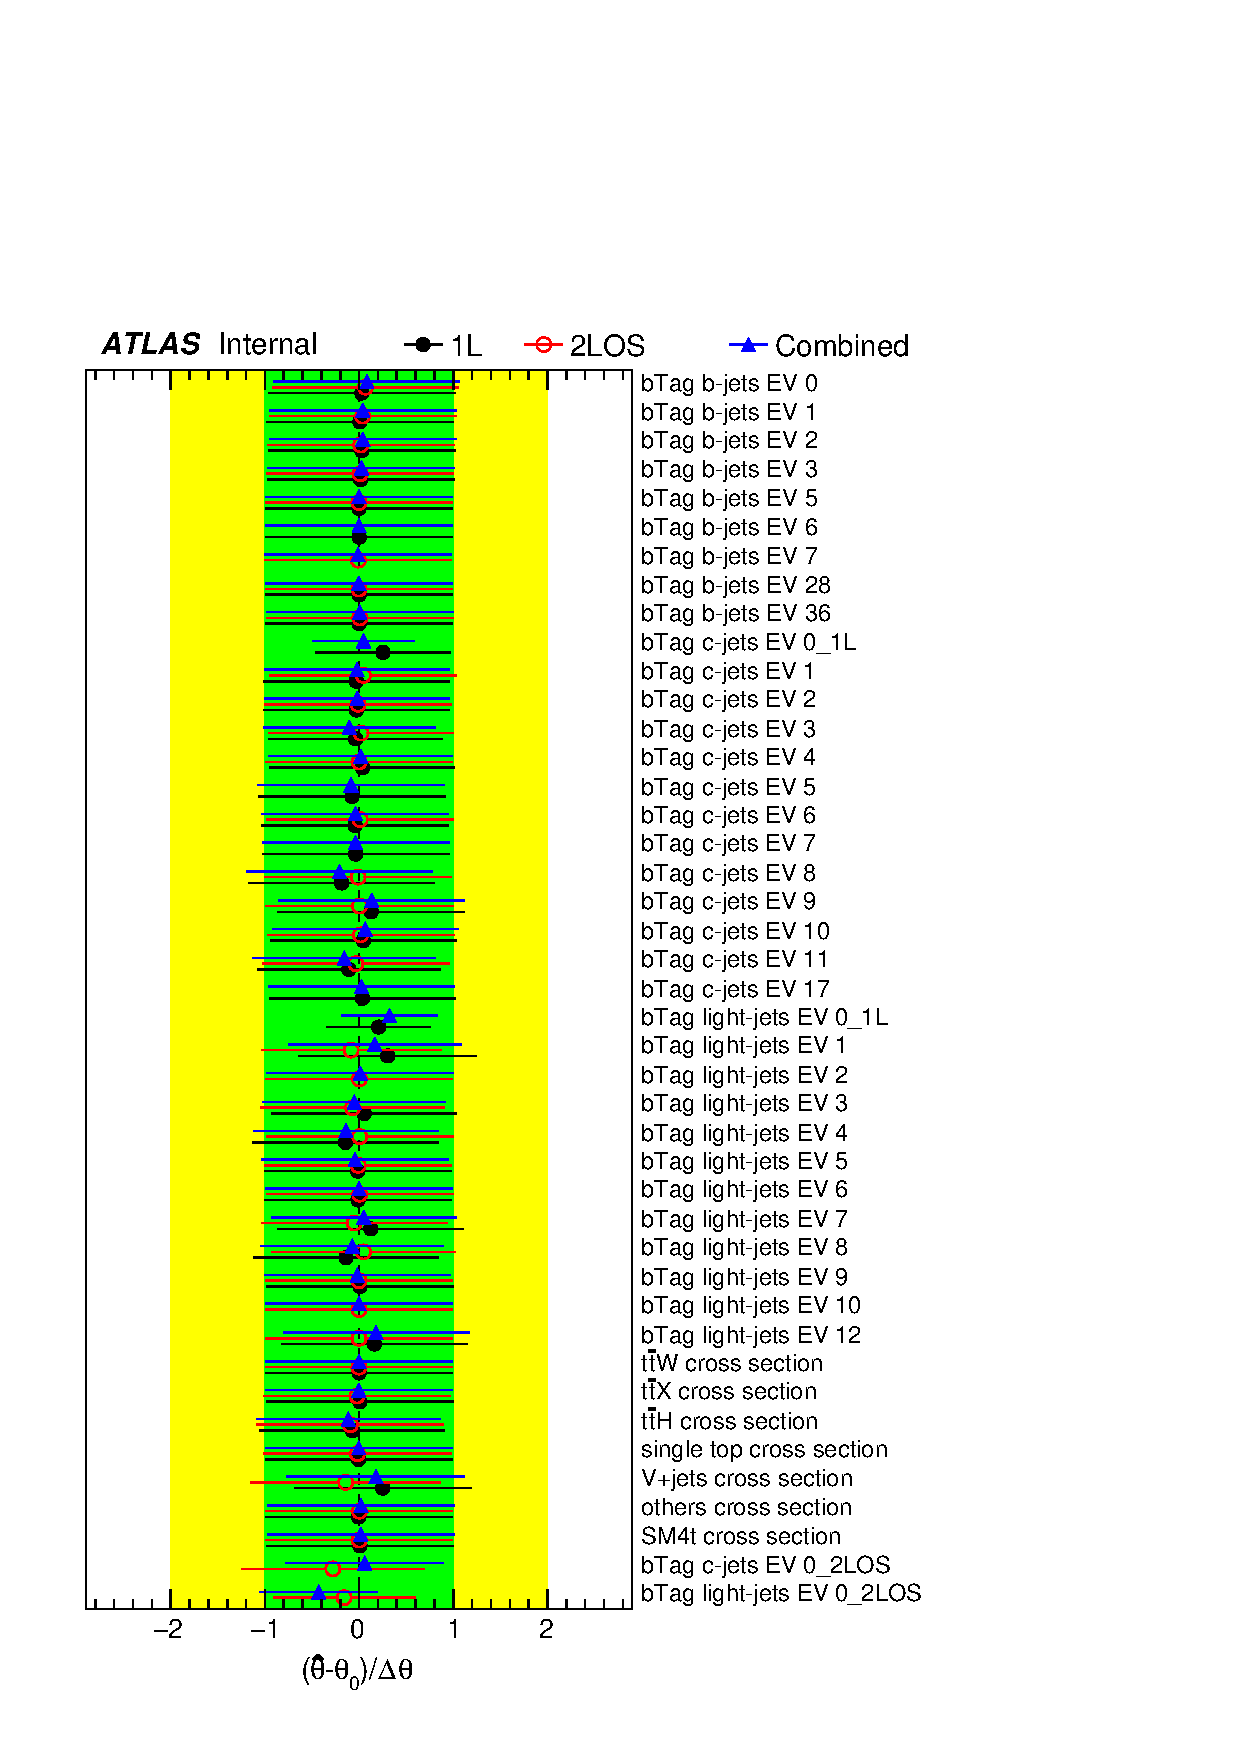
\includegraphics[width=0.58\textwidth]{plots/bkg_modelling/HF_scaling/PullPlots_multiFit.pdf}
    \end{subfigure}
    \caption{Fitted normalisation factors and nuisance parameters. Black, red and blue color refer to 1L, OS and combined channel fit respectively.}
    \label{fig:HF_scale_fit}
\end{figure}



The HF scale factors used in this analysis for the nominal \ttbar sample are taken as the normalization factors from Figure \ref{fig:HF_scale_fit}. It was found that the ratio $\ttbar_{postfit}^{nominal} / \ttbar_{prefit}^{nominal}$ based on Tables~\ref{tab:HF_preFit} and \ref{tab:HF_postFit_nominal} is very similar to the obtained normalization factors (1.18 for \ttbin, 1.60 for \ttcin, 0.83 for TTL (1L), and  0.87 for TTL (2L)).

The HF scale factors for the alternative \ttbar\ samples are obtained as the ratio $\ttbar_{postfit}^{nominal} / \ttbar_{prefit}^{alternative}$ based on the Tables~\ref{tab:HF_preFit} and \ref{tab:HF_postFit_nominal}. This is the preferred option because it also contains effects from the pulls from all nuisance parameters (it makes no difference for the nominal sample). No separate fits with alternative samples were used because they lead to large pulls on several nuisance parameters.  The HF scale factors of different \ttbar samples are summarized in table~\ref{tab:HF_results}. The \ttbar modelling systematics obtained using alternative weights in the nominal \ttbar sample (FSR, ISR, renormalization and factorization scale) are using the HF scale factors for the nominal \ttbar sample (the differences are negligible as documented in Appendix \ref{app:HFweights_weightSystematics}).


\begin{table}[!htb]
    \centering
    \resizebox*{0.72\textwidth}{!}{
    \begin{tabular}{c|c|c|c||c}
        \hline \hline
        \multicolumn{5}{c}{\textbf{Pre-fit 1L (Nominal)}}\\
        \hline
        & $LJETS,7j,2b$ & $LJETS,7j,3b$ & $LJETS,7j,\geq 4b$ & Total \\
        \hline 
TTL &  $132532.64 \pm 4215.99 $ & $5751.48 \pm 470.26$ & $44.24 \pm 11.26$ & $138328.36 \pm 4242.15$\\
TTC & $32634.67 \pm 888.81$ & $4491.35 \pm 360.70$ & $181.26 \pm 27.45$ & $37307.28 \pm 959.60$ \\
TTB & $14525.10 \pm 17.06$ & $9577.63 \pm 12.25$ & $2016.50 \pm 4.30$ & $26119.23 \pm 21.44$ \\ 
        \hline \hline
        \multicolumn{5}{c}{\textbf{Pre-fit OS (Nominal)}}\\
        \hline
        & $OS2L,5j,2b$ & $OS2L,5j,3b$ & $OS2L,5j,\geq 4b$ & Total \\
        \hline 
TTL &  $31869.24 \pm 961.92$ & $189.42 \pm 38.91$ & $0.51 \pm 0.26$ & $32059.17 \pm 962.71$\\
TTC & $6015.13\pm 150.02$ & $645.69 \pm 52.96$ & $10.95 \pm 1.71$ & $6671.77 \pm 159.10$  \\
TTB & $2994.50 \pm 5.91$ & $1870.36 \pm 4.24$ & $296.20 \pm 1.36$ & $5161.06 \pm 7.40$ \\
        \hline \hline \hline
        \multicolumn{5}{c}{\textbf{Pre-fit 1L (ttbb 4FS)}}\\
        \hline
        & $LJETS,7j,2b$ & $LJETS,7j,3b$ & $LJETS,7j,\geq 4b$ & Total \\
        \hline
TTL &  $132532.64 \pm 4215.99 $ & $5751.48 \pm 470.26$ & $44.24 \pm 11.26$ & $138328.36 \pm 4242.15$\\
TTC & $32634.67 \pm 888.81$ & $4491.35 \pm 360.70$ & $181.26 \pm 27.45$ & $37307.28 \pm 959.60$ \\
TTB & $14395.47 \pm 27.52$ & $9852.50 \pm 22.34$ & $2180.87 \pm 10.15$ & $26428.84 \pm 36.87$ \\
        \hline \hline
        \multicolumn{5}{c}{\textbf{Pre-fit OS (ttbb 4FS)}}\\
        \hline
         & $OS2L,5j,2b$ & $OS2L,5j,3b$ & $OS2L,5j,\geq 4b$ & Total \\
        \hline
TTL &  $31869.24 \pm 961.92$ & $189.42 \pm 38.91$ & $0.51 \pm 0.26$ & $32059.17 \pm 962.71$\\
TTC & $6015.13\pm 150.02$ & $645.69 \pm 52.96$ & $10.95 \pm 1.71$ & $6671.77 \pm 159.10$  \\
TTB & $2898.23 \pm 9.00$ & $1843.86 \pm 6.87$ & $309.36 \pm 2.65$ & $5051.45 \pm 11.63$ \\
        \hline \hline \hline
        \multicolumn{5}{c}{\textbf{Pre-fit 1L (aMcAtNloPy8)}}\\
        \hline
        & $LJETS,7j,2b$ & $LJETS,7j,3b$ & $LJETS,7j,\geq 4b$ & Total \\
        \hline
TTL & $117273.46 \pm 3716.78$ & $5116.16 \pm 420.24$ & $38.65 \pm 10.28$ & $122428.27 \pm 3740.48$\\
TTC & $29348.28 \pm 809.43$ & $3924.70 \pm 314.28$ & $151.22 \pm 22.69$ & $33424.20 \pm 868.60$  \\
TTB & $13398.83 \pm 38.45$ & $8851.56 \pm 27.21$ & $1913.43 \pm 8.88$ & $24163.82 \pm 47.93$ \\
        \hline \hline
        \multicolumn{5}{c}{\textbf{Pre-fit OS (aMcAtNloPy8)}}\\
        \hline
        & $OS2L,5j,2b$ & $OS2L,5j,3b$ & $OS2L,5j,\geq 4b$ & Total \\
        \hline
TTL &  $28880.01 \pm 889.56$ & $160.68 \pm 33.08$ & $0.72 \pm 0.40$ & $29041.41 \pm 890.17$ \\
TTC & $5565.00 \pm 140.81$ & $593.38 \pm 48.86$ & $9.58 \pm 1.60$ & $6167.96 \pm 149.05$\\
TTB & $2828.95 \pm 11.79$ & $1772.51 \pm 8.41$ & $296.82 \pm 2.72$ & $4898.28 \pm 14.74$\\
        \hline \hline \hline
        \multicolumn{5}{c}{\textbf{Pre-fit 1L (PhHerwig)}}\\
        \hline 
 & $LJETS,7j,2b$ & $LJETS,7j,3b$ & $LJETS,7j,\geq 4b$ & Total \\
        \hline
TTL & $166159.84 \pm 5232.84$ & $7001.95 \pm 573.57$ & $52.10 \pm 13.60$ & $173213.89 \pm 5264.20$ \\
TTC & $23306.84 \pm 635.75$ & $3190.58 \pm 255.02$ & $125.72 \pm 18.59$ & $26623.14 \pm 685.24$ \\
TTB & $11965.54 \pm 19.36$ & $7104.79 \pm 13.27$ & $1346.67 \pm 4.30$ & $20417.00 \pm 23.86$ \\ 
        \hline \hline
        \multicolumn{5}{c}{\textbf{Pre-fit OS (PhHerwig)}}\\
        \hline
 & $OS2L,5j,2b$ & $OS2L,5j,3b$ & $OS2L,5j,\geq 4b$ & Total \\
        \hline
TTL & $38019.17 \pm 1160.60$ & $199.01 \pm 40.78$ & $0.95 \pm 0.46$ & $38219.13 \pm 1161.32$ \\
TTC & $4689.39 \pm 118.92$ & $494.01 \pm 40.09$ & $7.17 \pm 1.09$ & $5190.57 \pm 125.50$ \\
TTB & $1845.12 \pm 5.22$ & $1184.89 \pm 3.62$ & $204.56 \pm 1.20$ & $3234.57 \pm 6.46$ \\ 
       \hline \hline
    \end{tabular}
    }
    \caption{\label{tab:HF_preFit}The pre-fit yields before the HF rescaling fit of different MC samples.}\end{table}

\begin{table}[!htb]
    \centering
    \resizebox*{0.72\textwidth}{!}{
    \begin{tabular}{c|c|c|c||c}
        \hline \hline
        \multicolumn{5}{c}{\textbf{Post-fit 1L (Nominal)}}\\
        \hline
        & $LJETS,7j,2b$ & $LJETS,7j,3b$ & $LJETS,7j,\geq 4b$ & Total \\
        \hline
TTL &  $109830.98 \pm 4123.96$ & $4709.29\pm 186.97$ & $34.41 \pm 2.65$ & $114574.68 \pm 4128.20$ \\
TTC & $52241.19 \pm 4105.77$ & $7145.79 \pm 557.11$ & $286.59 \pm 22.83$ & $59673.57 \pm 4143.46$ \\
TTB & $17153.71 \pm 403.20$ & $11310.90 \pm 265.87$ & $2381.43 \pm 55.98$ & $30846.04 \pm 486.20$\\
        \hline \hline
        \multicolumn{5}{c}{\textbf{Post-fit OS (Nominal)}}\\
        \hline
        & $OS2L,5j,2b$ & $OS2L,5j,3b$ & $OS2L,5j,\geq 4b$ & Total \\
        \hline
TTL & $27717.06 \pm 794.56$ & $178.53 \pm 26.36$ & $0.53 \pm 0.18$ & $27896.12 \pm 795.00$\\
TTC &  $9707.14 \pm 703.54$ & $1039.12 \pm 63.97$ & $17.83 \pm 1.62$ &  $10764.09 \pm 706.44$ \\
TTB & $3536.52 \pm 83.14$ & $2208.95 \pm 51.92$ & $349.84 \pm 8.24$ & $6095.31 \pm 98.37$ \\
        \hline \hline
    \end{tabular}
    }
    \caption{\label{tab:HF_postFit_nominal}The post-fit yields after the HF rescaling fit on the nominal MC samples.}
\end{table}

\begin{table}[!htb]
    \centering
    \resizebox*{0.5\textwidth}{!}{
    \begin{tabular}{c|cccc}
        \hline \hline
        & TTL (1L) & TTL (OS) & TTC & TTB \\
        Nominal & $0.84\pm 0.04$ & $0.87\pm 0.03$ & $1.61\pm 0.13$ & $1.18\pm 0.03$\\
        ttbb 4FS & $0.83\pm 0.04$ & $0.87\pm 0.04$ & $1.60\pm 0.10$ & $1.17\pm 0.02$ \\
        aMcAtNloPy8 & $0.94\pm 0.04$ & $0.96\pm 0.04$ & $1.78\pm 0.11$ & $1.27\pm 0.01$\\
        PhHerwig & $0.66\pm 0.03$ & $0.73\pm 0.03$ & $2.21\pm 0.14$ & $1.56\pm 0.02$ \\ 
        \hline \hline
    \end{tabular}
    }
    \caption{\label{tab:HF_results}The summary of HF scale factors of TTL (1L and OS), TTC and TTB of different \ttbar+jets MC samples.}
\end{table}
